\documentclass[a4paper]{article}

\usepackage[rowmode]{ticket}
\usepackage[margin=5mm]{geometry}
\usepackage{graphicx,pst-all}
\usepackage{fontspec,newunicodechar}
\usepackage{enumitem}
\setlist{nosep,font=\textbf,align=left, leftmargin=1em,
labelindent=\parindent, listparindent=\parindent, labelwidth=0pt,
labelsep=1em, itemindent=!}
\setmainfont[Path=../fonts/,UprightFont=*.otf,BoldItalicFont=*Exp-Italic.otf,BoldFont=*-Bold.otf,ItalicFont=*-Italic.otf,SmallCapsFont=*-Bold.otf]{D-DIN}
\setsansfont[Path=../fonts/,UprightFont=*.otf,BoldItalicFont=*-Bold.otf,BoldFont=*-Bold.otf]{D-DINCondensed}
\newunicodechar{⁰}{{${}^{\it 0}$}}
\newunicodechar{¹}{{${}^{\it 1}$}}
\newunicodechar{²}{{${}^{\it 2}$}}
\newunicodechar{³}{{${}^{\it 3}$}}
\newunicodechar{⁴}{{${}^{\it 4}$}}
\newunicodechar{⁵}{{${}^{\it 5}$}}
\newunicodechar{⁶}{{${}^{\it 6}$}}
\newunicodechar{⁷}{{${}^{\it 7}$}}
\newunicodechar{⁸}{{${}^{\it 8}$}}
\newunicodechar{⁹}{{${}^{\it 9}$}}

\definecolor{darkgreen}{rgb}{0,0.5,0}
\setlength{\unitlength}{1mm}
\psset{unit=1mm}
\ticketNumbers{3}{3}
\ticketSize{60}{90}
\ticketDistance{10}{5}

\newcommand{\propertyline}[2]{%
  \psframe(0,0)(52,5)
  \rput[tl](1,4){\textsf{#1\phantom{Q}}}%
  \rput[tr](51,4){\phantom{Q}#2}%
  % the Phantom Qs fix line height alignment issues; Q extends to
  % uppermost and lowermost vertical positions.
}

\newcommand{\others}[2]{%
  \psframe[fillcolor=#2](0,0)(12,-2)
  \rput[tc](6,-1){\tiny\phantom{Q}#1\phantom{Q}}
}

\renewcommand{\ticketdefault}{}

\newcommand{\titleticket}{\ticket{%
  \begin{pspicture}(0,0)(60,90)
    \psset{cornersize=absolute}
    % cut frame for the cards:
    \psframe[linewidth=1pt,linearc=6,fillstyle=none,linestyle=dotted](0,0)(60,90)
    % printed card frame
    \psboxfill{\includegraphics[width=54mm,height=84mm]{../pictures/titel.jpg}}
    \psframe[linearc=3,fillstyle=boxfill,fillsize={(3mm,3mm)(54mm,84mm)}](3,3)(57,87)
    \psframe[linearc=2,fillstyle=none,linestyle=solid,linecolor=white,linewidth=.3mm](4,4)(56,86)
    \rput[t](30,80){\Huge \color{white}\textbf{Triebwagen-}}
    \rput[t](30,20){\Huge \color{white}\textbf{quartett}}
  \end{pspicture}
}}

\newcommand{\copyrightticket}{\ticket{%
  \begin{pspicture}(0,0)(60,90)
    \psset{cornersize=absolute}
    \psset{fillstyle=none}
    % cut frame for the cards:
    \psframe[linewidth=1pt,linearc=6,linestyle=dotted](0,0)(60,90)
    % printed card frame
    \psframe[linearc=3](3,3)(57,87)
    \rput[tc](30,84){\textbf{Urheberrecht}}
    \rput[tr](54,84){\includegraphics[width=10mm]{../by-sa.eps}}
    \rput[tl](4,80){
    \begin{minipage}{50mm}
      \tiny
      Dieses Quartett ist © CC BY-SA 4.0 Bjørn Bäuchle.\\
      Die folgenden Bilder stehen unter abweichenden Lizenzen:
      \begin{itemize}
        \item[Desiro HC] Von RomainDil - Eigenes Werk, CC~BY-SA 4.0,\\
  https://commons.wikimedia.org/w/index.php?curid=78177186
\item[Desiro ML] Von Rob Dammers - Köln Messe-Deutz Transregio 460~011-460~007 RB25 Mainz Hbf, CC~BY 2.0,\\
  https://commons.wikimedia.org/w/index.php?curid=66189854
\item[ET0423] Von MdE - Eigenes Foto, CC~BY-SA 3.0 de,\\
   https://commons.wikimedia.org/w/index.php?curid=9858236
\item[ET0430] Von Peter Stehlik PS-2507 - Eigenes Werk, CC~BY-SA 3.0,\\
   https://commons.wikimedia.org/w/index.php?curid=31896378
\item[FLIRT 3XL] CC BY-SA 4.0 lostAm
\item[ICE 2] Von Sebastian Terfloth User:Sese\_Ingolstadt - Eigenes Werk, CC~BY-SA 3.0,\\
  https://commons.wikimedia.org/w/index.php?curid=3888160
\item[ICE 3MS] Von Nicky Boogaard -\\
  https://www.flickr.com/photos/n-bphotography/40747719593/, CC~BY 2.0,\\
  https://commons.wikimedia.org/w/index.php?curid=81962027
\item[iLINT 54] Von MdE - Eigenes Foto, CC~BY-SA 3.0 de,\\
  https://commons.wikimedia.org/w/index.php?curid=128843100
\item[Integral] Von Constantin A. - Eigenes Werk, CC BY-SA 4.0
\item[KISS 160] Von Clic - Eigenes Werk, CC~BY-SA 4.0,\\
   https://commons.wikimedia.org/w/index.php?curid=67194026
\item[KISS 200] Von Boevaya mashina - Eigenes Werk, CC~BY-SA 4.0,\\
   https://commons.wikimedia.org/w/index.php?curid=92097473
\item[Mireo] Von Maximilian Wegner - Eigenes Werk, CC~BY-SA 4.0,
  https://commons.wikimedia.org/w/index.php?curid=114050699
\item[RegioSprinter] Von Alupus - Eigenes Werk, CC~BY-SA 3.0,\\
  https://commons.wikimedia.org/w/index.php?curid=16103573
\item[TALENT 2] Von Falk2 - Eigenes Werk, CC~BY-SA 4.0,\\
  https://commons.wikimedia.org/w/index.php?curid=45335615
\item[TwinDexx Vario] Von Falk2 - Eigenes Werk, CC~BY-SA 3.0 de,\\
   https://commons.wikimedia.org/w/index.php?curid=86667724

      \end{itemize}
      \smallskip
      Detaillierte Informationen und alle Quelltexte sind unter
      https://github.com/baeuchle/triebwagen\_quartett/ verfügbar.
    \end{minipage}
  }
  \end{pspicture}
}}

\newcommand{\quartettkarte}[9]{%
  \def\tempNummer{#1}%
  \def\tempName{#2}%
  \def\tempDesc{#3}%
  \def\tempFile{#4}%
  \def\tempBild{\includegraphics[width=50mm,height=30mm]{../pictures/#4}}%
  \def\tempSitzplaetze{#5}%
  \def\tempLaenge{#6}%
  \def\tempTeile{#7}%
  \def\tempAchsen{#8}%
  \def\tempLeistung{#9}%
  \kartecontinued%
}
\newcommand{\kartecontinued}[7]{\ticket{%
  \def\tempVmax{#1}%
  \def\tempMasse{#2}%
  \def\tempEins{#3}%
  \def\tempZwei{#4}%
  \def\tempDrei{#5}%
  \def\tempVier{#6}%
  \begin{pspicture}(0,0)(60,90)
    \psset{cornersize=absolute}
    % cut frame for the cards:
    \psframe[linewidth=1pt,linearc=6,fillstyle=none,linestyle=dotted](0,0)(60,90)
    % printed card frame
    \psset{fillstyle=solid}
    \psframe[linearc=3,fillcolor=gray](3,3)(57,87)
    \multido{\n=5.0+1.9}{20}{
      \rput(3.00,\n){\psCoil[coilaspect=0,coilheight=10.8,coilwidth=1.0,linewidth=.15pt,linecolor=white]{0}{1800}}
    }
    \multido{\n=45.7+1.9}{21}{
      \rput(3.00,\n){\psCoil[coilaspect=0,coilheight=10.8,coilwidth=1.0,linewidth=.15pt,linecolor=white]{0}{1800}}
    }
    \psframe[linearc=3,fillstyle=none](3,3)(57,87)
    % headline:
    \psset{fillcolor=white}
    \psset{linestyle=none}
    % only left upper corner is rounded:
    \psframe[linearc=2](4,77)(43,86)
    \psframe(4,77)(7,80)
    \psframe(39,77)(43,86)
    \rput(23.5,81.5){\textbf{\large \tempName}}
    % only right upper corner is rounded;
    \psframe[linearc=2](44,77)(56,86)
    \psframe(44,77)(47,86)
    \psframe(53,77)(56,80)
    \rput[t](50,84.5){\textbf{\Huge \tempNummer}}
    \rput[tl](5,76){\tempBild}
    \rput[tc](30,44){\textit{\color{yellow}\textbf{\tempDesc}}}
    {% data
      \rput(4,36){\propertyline{Sitzplätze}{\tempSitzplaetze}}
      \rput(4,30){\propertyline{Länge}{\tempLaenge{} m}}
      \rput(4,24){\propertyline{Fahrgastteile/Achsen}{\tempTeile/\tempAchsen}}
      \rput(4,18){\propertyline{Leistung}{\tempLeistung{} MW}}
      \rput(4,12){\propertyline{Höchstgeschwindigkeit}{\tempVmax{} km/h}}
      \rput(4,6){ \propertyline{Leermasse}{\tempMasse{} t}}
    }
  \rput[tl](6,6){% other cards from same letter
    \rput[tl](00,0){\others{\tempEins}{yellow}}
    \rput[tl](12,0){\others{\tempZwei}{green}}
    \rput[tl](24,0){\others{\tempDrei}{cyan}}
    \rput[tl](36,0){\others{\tempVier}{lime}}
  }
  \end{pspicture}
}}
\newcommand{\rueckseite}{\ticket{%
  \begin{pspicture}(0,0)(60,90)
    \psset{cornersize=absolute}
    \psset{fillstyle=none}
    % cut frame for the cards:
    \psframe[linewidth=1pt,linearc=6,linestyle=dotted](0,0)(60,90)
    % printed card frame
    \psboxfill{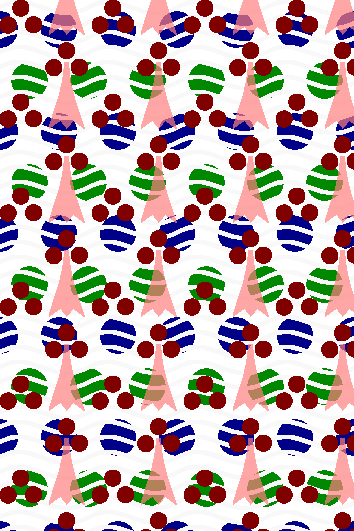
\includegraphics[width=54mm,height=84mm]{../pictures/background.pdf}}
    \psframe[linearc=3,linestyle=solid,linewidth=1mm,linecolor=black,fillstyle=boxfill,fillsize={(3mm,3mm)(54mm,84mm)}](3,3)(57,87)
  \end{pspicture}
}}

\begin{document}
\titleticket
\copyrightticket
\quartettkarte{}{}{}{fehlt.pdf}%
    {}{}{}{\phantom{99}}{}{}{}%
    {}{}{}{}{}
%%%%%%%%%%%%%%%%%%%%%%%%
\quartettkarte{A1}{Coradia A TER}{VT 0641}{vt0641.jpg}%
    {63}{28,9}{1}{4}{0,51}{120}{49}%
    {Coradia A TER}{RegioSprinter}{RegioShuttle}{GTW 2/6}{}%
\quartettkarte{A2}{RegioSprinter}{VT 0654}{vt0654.jpg}%
    {74}{24,8}{3}{4}{0,40}{120}{49}%
    {Coradia A TER}{RegioSprinter}{RegioShuttle}{GTW 2/6}{}%
\quartettkarte{A3}{RegioShuttle}{VT 0650}{vt0650.jpg}%
    {101}{25,5}{1}{4}{0,53}{120}{40}%
    {Coradia A TER}{RegioSprinter}{RegioShuttle}{GTW 2/6}{}%
\quartettkarte{A4}{GTW 2/6}{VT 0646}{vt0646.jpg}%
    {120}{38,7}{2}{6}{0,42}{120}{52}%
    {Coradia A TER}{RegioSprinter}{RegioShuttle}{GTW 2/6}{}%
%%%%%%%%%%%%%%%%%%%%%%%%
\quartettkarte{B1}{PESA LINK}{633⁰{\tiny + 933⁰ + }633⁵}{vt0633.jpg}%
    {106}{57,1}{3}{8}{1,13}{140}{120}%
    {PESA LINK}{Integral}{LINT 41}{Desiro Classic}{}
\quartettkarte{B2}{Integral}{VT 0609¹}{vt0609-1.jpg}%
    {164}{53,4}{5}{6}{0,95}{140}{74}%
    {PESA LINK}{Integral}{LINT 41}{Desiro Classic}{}
\quartettkarte{B3}{LINT 41}{VT 0648}{vt0648.jpg}%
    {120}{41,8}{2}{6}{0,80}{120}{63}%
    {PESA LINK}{Integral}{LINT 41}{Desiro Classic}{}
\quartettkarte{B4}{Desiro Classic}{VT 0642}{vt0642.jpg}%
    {110}{41,7}{2}{6}{0,72}{120}{69}%
    {PESA LINK}{Integral}{LINT 41}{Desiro Classic}{}
    %%%%%%%%%%%%%%%%%%%%%%%%
\quartettkarte{C1}{TALENT 1}{643⁰{\tiny + 943⁰ + }643⁵}{vt0643.jpg}%
    {137}{48,4}{3}{8}{0,63}{120}{72}%
    {TALENT 1}{Itino}{iLINT 54}{RegioSwinger}{}
\quartettkarte{C2}{Itino}{VT 0615}{vt0615.jpg}%
    {119}{39,5}{2}{6}{1,14}{140}{62}%
    {TALENT 1}{Itino}{iLINT 54}{RegioSwinger}{}
\quartettkarte{C3}{iLINT 54}{ETH 0554}{eth554.jpg}%
    {138}{54,3}{2}{8}{0,54}{120}{98}%
    {TALENT 1}{Itino}{iLINT 54}{RegioSwinger}{}
\quartettkarte{C4}{VT 0612}{RegioSwinger \tiny Neigetechnik}{vt0612.jpg}%
    {146}{51,8}{2}{8}{1,13}{160}{116}%
    {TALENT 1}{Itino}{iLINT 54}{RegioSwinger}{}
%%%%%%%%%%%%%%%%%%%%%%%%
\quartettkarte{D1}{ET 0423}{423⁰{\tiny + 433⁰ + 433⁵ + }423⁵}{et0423.jpg}%
    {192}{67,4}{4}{10}{2,35}{140}{105}%
    {423}{430}{RegioTram}{426}{}
\quartettkarte{D2}{ET 0430}{430⁰{\tiny + 431⁰ + 431⁵ + }430⁵}{et0430.jpg}%
    {184}{68,3}{4}{10}{2,35}{140}{119}%
    {423}{430}{RegioTram}{426}{}
\quartettkarte{D3}{RegioTram E+E}{452⁷{\tiny + 452⁵ + }852⁷}{et0452.jpg}%
    {90}{37,5}{3}{8}{0,60}{100}{60}%
    {423}{430}{RegioTram}{426}{}
\quartettkarte{D4}{ET 0426}{426⁰ + 426⁵, \tiny 425⁰+435⁰+435⁵+425⁵}{et0426.jpg}%
    {100}{36,5}{2}{6}{1,18}{160}{63}%
    {423}{430}{RegioTram}{426}{}
%%%%%%%%%%%%%%%%%%%%%%%%
\quartettkarte{E1}{FLIRT 1 (4-tlg)}{0428⁰{\tiny + 0828⁰ + 0828⁵ + }0428⁵}{et0428.jpg}
    {219}{74,3}{4}{10}{2,00}{160}{120}%
    {FLIRT 1}{FLIRT 3XL}{Desiro ML}{Mireo}{}
\quartettkarte{E2}{FLIRT 3XL (3-tlg)}{3427⁰{\tiny + 3827⁰ + }3427⁵}{et3427.jpg}%
    {181}{67,6}{3}{8}{2,00}{160}{100}%
    {FLIRT 1}{FLIRT 3XL}{Desiro ML}{Mireo}{}
\quartettkarte{E3}{Desiro ML}{ET 0460}{et0460.jpg}
    {252}{70,9}{3}{12}{2,60}{160}{132}%
    {FLIRT 1}{FLIRT 3XL}{Desiro ML}{Mireo}{}
\quartettkarte{E4}{Mireo}{ET 0463, \tiny ETH0563}{et0463.jpg}
    {160}{72,0}{3}{8}{2,6}{160}{101}% % Länge geraten
    {FLIRT 1}{FLIRT 3XL}{Desiro ML}{Mireo}{}
%%%%%%%%%%%%%%%%%%%%%%%%
\quartettkarte{F1}{TALENT 2}{ET 9442}{et9442.jpg}
    {162}{56,2}{3}{8}{2,28}{160}{103}% % Sitzplätze und Leermasse geraten
    {TALENT 2}{Continental}{Desiro HC}{TwinDexx Vario}{}
\quartettkarte{F2}{Coradia Continental}{1440²{\tiny + 1441² + 1841² + 1441⁷ + }1440⁷}{et1440.jpg}
    {293}{89,7}{5}{12}{2,88}{160}{168}%
    {Mireo}{Desiro ML}{Continental}{TALENT 2}{}
\quartettkarte{F3}{Desiro HC}{ET 0462}{et0462.jpg}%
    {400}{105,3}{4}{16}{4,00}{160}{198}%
    {Desiro HC}{TwinDexx Vario}{KISS 160}{FLIRT 1}{}
\quartettkarte{F4}{TwinDexx Vario}{445{\tiny + DBpza + DABpza + }445}{et0445.jpg}%
    {437}{105,6}{4}{16}{4,60}{160}{227}%
    {Desiro HC}{TwinDexx Vario}{KISS 160}{FLIRT 1}{}
%%%%%%%%%%%%%%%%%%%%%%%%
\quartettkarte{G1}{KISS 160}{445⁰{\tiny + 446² + 446³ + 446⁴ + 446⁵ + 446⁶+ }445⁷}{et0446.jpg}%
    {626}{156,5}{6}{24}{4,50}{160}{296}%
    {KISS 160}{KISS 200}{ICE-T}{ICE 4}{}
\quartettkarte{G2}{KISS 200}{ET 4110}{et4110.jpg}%
    {302}{100,0}{4}{16}{4,00}{200}{218}%
    {KISS 160}{KISS 200}{ICE-T}{ICE 4}{}
\quartettkarte{G3}{ICE-T7}{T7: 5411, \small T5: 5415, TD4: VT 605}{et5411.jpg}%
    {376}{185,0}{7}{28}{4,00}{230}{386}%
    {KISS 160}{KISS 200}{ICE-T}{ICE 4}{}
\quartettkarte{G4}{ICE 4.13}{412, Tz 9450ff}{et0412.jpg}%
    {450}{374,0}{13}{52}{11,55}{265}{731}%
    {KISS 160}{KISS 200}{ICE-T}{ICE 4}{}
%%%%%%%%%%%%%%%%%%%%%%%%
\quartettkarte{H1}{ICE 1 LDV}{401,801-804 \small Tz 1xx}{et5401.jpg}%
    {503}{278,7}{9}{44}{9,60}{280}{627}%
    {ICE 1 LDV}{ICE 2}{ICE 3}{ICE 3MS}{}
\quartettkarte{H2}{ICE 2}{5402,805-808 {\small Tz 2xx}}{et5402.jpg}%
    {381}{205,4}{7}{32}{4,80}{280}{418}%
    {ICE 1 LDV}{ICE 2}{ICE 3}{ICE 3MS}{}
\quartettkarte{H3}{ICE 3}{5403 {\tiny Tz 3xx 1-System, 406: Tz 46xx 4-System}}{et5403.jpg}%
    {374}{200,8}{8}{32}{8,00}{330}{435}%
    {ICE 1 LDV}{ICE 2}{ICE 3}{ICE 3MS}{}
\quartettkarte{H4}{ICE 3 MS}{ET 5407 \small Tz 7xx}{et5407.jpg}%
    {444}{200,7}{8}{32}{8,00}{320}{463}%
    {ICE 1 LDV}{ICE 2}{ICE 3}{ICE 3MS}{}
%%%%%%%%%%%%%%%%%%%%%%%%
\quartettkarte{}{}{}{fehlt.pdf}%
    {}{}{}{\phantom{99}}{}{}{}%
    {}{}{}{}{}
% unused:
%\quartettkarte{}{LINT 81}{VT 0620}{vt0620.jpg}%
%    {300}{80,9}{3}{12}{1,56}{140}{138}%
%    {}{}{}{}{}%
%\quartettkarte{}{LINT 27}{VT 0640}{vt0640.jpg}%
%    {52}{27,3}{1}{4}{0,32}{120}{41}%
%    {}{}{}{}{}
\newpage\ticketreset
\newcounter{numcards}
\setcounter{numcards}{0}
\whiledo{\thenumcards<36}{\stepcounter{numcards}\rueckseite}
\end{document}
